\ignore{From real-case observations, we discover several relational
constraints among concept relations that can be used to enforce the
relation between two input concepts identified by our relation
classifier.} 

Analyzing concepts and the relations between them reveals several
relational constraints among the relations identified for the target
pair and those identified for related concepts. For instance, concept
{\em George W. Bush} cannot be an ancestor or sibling of concept {\em
  president} if we are confident that concept {\em president} is an
ancestor of concept {\em Bill Clinton}, and {\em Bill Clinton} is a
sibling of concept {\em George W. Bush}. Another example would be that
if concepts {\em red} and {\em green} are known to be siblings, and
concept {\em blue} is also known to be a sibling of {\em red}, the
prediction identifying that {\em green} is an ancestor of {\em blue}
should be invalid. We call the combination of concepts and their
relations {\em concept network}. Fig. \ref{fig:triangles} shows some
$n$-vertex concept networks consisting of two input concepts
($x$, $y$), and additional concepts $z$, $w$,
$v$. Fig. \ref{fig:triangles}(b) and \ref{fig:triangles}(d) illustrate
two relational constraints. In general, $n$ concepts can be involved
to construct $n$-vertex concept network ($n > 2$). In this paper, we
focus on observing $3$-vertex concept networks consisting of the two
input concepts and an additional one. However, our formalization
applies to general $n$-vertex concept networks.
% The problem of determining optimal value of $n$ is beyond the scope
% of this paper.

\ignore{From our observations, we see that if we can obtain additional
  concepts in addition to the two input concepts, we can enforce such
  relational constraints as prior knowledge to guide the final
  decision of the relation identifier. In the literature, several
  models take advantage of prior knowledge to achieve significant
  improvement in performance
  \cite{CGRT09,DenisBa07,PunyakanokRoYi05}. There are two main
  approaches to inject prior knowledge. The first approach
  incorporates prior knowledge {\em indirectly}; by adding more
  features \cite{RothYi05}. The other incorporates prior knowledge
  {\em directly} in the form of hard or soft constraints
  \cite{ChangRaRo08}. We want to incorporate prior knowledge directly,
  therefore our model is closely related to the latter approach.}

The aforementioned observations show that, if we can obtain additional
concepts that are related to the two input concepts, we can enforce
such relational constraints as prior knowledge and guide the final
decision of the relation identifier. Our formulation follows
constraint-based formulations that were introduced in the NLP
community and were shown to be very effective in exploiting
declarative background knowledge as a way to achieve significant
improvement in performance
\cite{RothYi04,PRYZ05,CGRT09,DenisBa07,PunyakanokRoYi05}. While it is
also possible to inject prior knowledge {\em indirectly}, by adding
more features, it has been argued (e.g., \cite{RothYi05,ChangRaRo08})
that a {\em direct} way, in the form of soft or hard constraints, is
beneficial due to better expressivity and simpler learning. Our model
follows this approach.

\begin{figure}[!t]
\centering
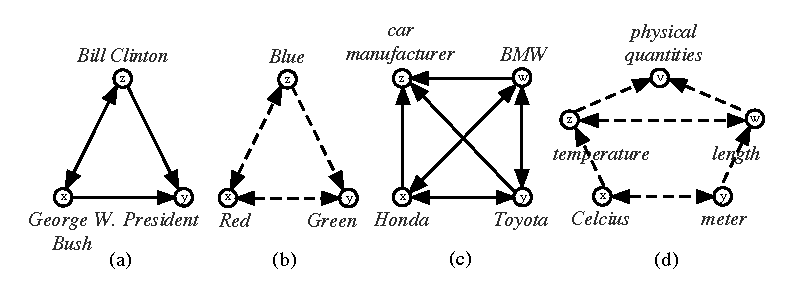
\includegraphics[totalheight=0.1\textheight]{networks}
\caption{Examples of $n$-vertex concept networks formed by two input
  concepts $x$, $y$, and related concept $z$, $w$ and $v$. The
  relation between concepts is predicted by a local classifier (see
  Sec. \ref{sec:learner}). Concept networks (a) and (c) show valid
  combinations of edges, whereas (b) and (d) demonstrate invalid
  combinations of edges. (b) and (d) form two relational constraints
  that we do not allow. For simplicity, we do not draw {\em no
    relation} edges in (d).}
\label{fig:triangles}
\end{figure}

\subsection{Constraints as Prior Knowledge}
\label{sec:cons-prior-know}
Let two input concepts $(x,y)$, and a set of additional concepts
$\mathcal{Z}^*=\{z_1, z_2, ..., z_m\}$.  For a subset $\mathcal{Z} \in
\mathcal{Z}^*$, a set of concept networks is constructed. Each concept
network contains two input concepts $x$, and $y$, and all additional
concepts in $\mathcal{Z}$. Every two concepts in a concept network are
connected by their relations which are the four relations of interest
in this paper. A local relation classifier is used to give weights for
4 relation classes of an edge in a concept network. We use $e$ and
$w(e)$ to denote an edge in a concept network and its corresponding
weight, respectively. If $n$ is the number of concepts in a network
($n > 2$), there will be $\left [ \frac{1}{2} n(n-1) \right ] ^4$
concept networks that can be constructed because there are $4$
relations for every $2$ concepts. For instance, with $n=3$, we have
$64$ concept networks.  A relational constraint is defined as an
invalid concept networks that is not allowed to happen. Figure
\ref{fig:triangles}(b) demonstrates a constraint where the combination
of edges is ({\em sibling}, {\em sibling}, {\em ancestor}) moving
clockwise direction with respect to $x$ and $y$.

Let $\mathcal{C}$ be a list of relational constraints. Following the
approaches to inject prior knowledge directly in \cite{ChangRaRo08}, we
incorporate relational constraints into our model to choose the best
network $t^*$ from a set of concept networks constructed from $\left <
  x, y, \mathcal{Z} \right >$. The scoring function is a linear
combination of the edge weights $w(e)$ and the penalties $\rho_k$ of
concept networks violating constraint $C_k \in \mathcal{C}$.

\begin{equation}
  \label{eqn:tscore}
  t^* = \text{argmax}_{t} \sum_{e \in t} w(e) - \sum_{k=1}^{|\mathcal{C}|} \rho_{k} d_{C_k}(t)
\end{equation}

In Eqn. \ref{eqn:tscore}, function $d_{C_k}(t)$ measures the degree
that concept network $t$ violates constraint $C_k$.  In our work,
relational constraints are mined from the training data (see
Sec. \ref{sec:constraintselection}). Therefore, the selected
constraints are considered to have high confidence. We, thus, use them
as hard constraints and set their penalty $\rho_k$ to $\infty$
\cite{ChangRaRo08}. Objective function \ref{eqn:tscore} allows us to
pick the best setting of all edges connecting concepts in the networks
with respect to relational constraints.

After having the model to choose the topmost concept network for a
particular subset of additional concepts $\mathcal{Z} \in
\mathcal{Z}^*$, we are going to make the final decision on the
relation between $x$ and $y$. Note that for each subset of additional
concepts $\mathcal{Z} \in \mathcal{Z}^*$, the topmost concept network
contains the most likely relation $\ell$ of the two input concepts $x$
and $y$. After collecting all the topmost concept networks by going
through all $\mathcal{Z} \in \mathcal{Z}^*$, the topmost concept
networks are divided into four group with respect to the relation of
$x$ and $y$ in each network. Each group of the topmost concept
networks is denoted by $\mathcal{T}_{\ell}$. To make the final
decision concerning the relation of two input concepts $(x,y$), we
solve the objective function defined in
Eqn. \ref{eqn:objectivefunction}.

\begin{eqnarray}
\label{eqn:objectivefunction}
\ell^* & = & \text{argmax}_{\ell} \frac {1} {|\mathcal{T}_{\ell}|} \sum_{t \in \mathcal{T}_{\ell}} \lambda_{t} score(t) \\
& = & \text{argmax}_{\ell} \frac{1}{|\mathcal{T}_{\ell}|} \sum_{t \in \mathcal{T}_{\ell}} \lambda_{t} \left( \sum_{e \in t} w(e) - \sum_{k=1}^{|\mathcal{C}|} \rho_{k} d_{C_k}(t) \right) \notag
\end{eqnarray}

where 

\begin{equation}
  \lambda_t = \frac{\# \text{ of occurrences of }t}{\# \text{ of
      predicted concept networks in training data}} \notag
\end{equation}

is the occurrence probability of concept network $t$ in the training
data with additional concepts. To measure $\lambda_t$, a local
relation classifier is used to predict the best relation between
concepts in the concept networks in the training data.

\subsection{Constraint Selection}
\label{sec:constraintselection}

In Eqn. (\ref{eqn:objectivefunction}), a list of relational
constraints $\mathcal{C}$ is used. Recall that a relational constraint
is an invalid concept network that is not allowed to happen. In our
work, relational constraints are mined from the training data by
applying the {\em forward feature selection} technique discussed in
\cite{944968}. The algorithm starts with an empty set of constraints
$\mathcal{C}$, then grows the constraint set gradually by including in
the set the {\em best} concept network from each iteration. The {\em
  best} concept network is defined as the constraint used in
Eqn. (\ref{eqn:objectivefunction}) that improves the system's
performance most. Our {\em forward constraint selection} algorithm is
described in Fig. \ref{alg:forwardselection}. Function
\texttt{evaluate}($\mathcal{D}$, $\mathcal{L}$, $\mathcal{C}$)
evaluates the system on all examples and their related concepts in
$\mathcal{D}$ using a trained local classifier $\mathcal{L}$ with
respect to a set of constraints $\mathcal{C}$ by solving the objective
function in Eqn. (\ref{eqn:objectivefunction})

\begin{figure}[!t]
  \begin{centering}
    {\scriptsize
      \fbox{
        \begin{minipage}{6in} 
          \begin{tabbing}
            {Algorithm \textsc{Forward Constraint Selection}} \\
            \qquad {\textsc{Input}}: Data set with related concepts $\mathcal{D} = \left < (x, y, \ell, \mathcal{Z}^*) \right >$ ~~~~~\\
            \qquad \qquad A trained local relation classifier $\mathcal{L}$. \\
            \qquad \qquad A list of concept networks $\mathcal{T} = \{ t_1, t_2, \dots, t_{m} \}$; \\
            \qquad {\textsc{Output}}: Constraint set $\mathcal{C}$. \\
            \\
            \qquad $\mathcal{C} = \emptyset$; {\em isIncreasing} = true; \\
            \qquad {\em bestAcc} = \texttt{evaluate}($\mathcal{D}$, $\mathcal{L}$, $\mathcal{C}$); \\
            \qquad While ({\em isIncreasing}) do \\
            \qquad \qquad {\em isIncreasing} = false; \\
            \qquad \qquad For each $t \in \mathcal{T}$ do \\
            \qquad \qquad \qquad $\mathcal{C} = \mathcal{C} \cup \{ t \}$; \\
            \qquad \qquad \qquad {\em acc} = \texttt{evaluates}($\mathcal{D}$, $\mathcal{L}$, $\mathcal{C}$); \\
            \qquad \qquad \qquad If ({\em acc} $>$ {\em bestAcc}) then \\ 
            \qquad \qquad \qquad \qquad $t^* = t$; {\em isIncreasing} = true; \\ 
            \qquad \qquad \qquad \qquad {\em bestAcc} $=$ {\em acc}; \\ 
            \qquad \qquad \qquad End if \\ 
            \qquad \qquad \qquad $\mathcal{C} = \mathcal{C} \backslash \{ t \}$; \\
            \qquad \qquad End for \\
            \qquad \qquad If ({\em isIncreasing}) then \\
            \qquad \qquad \qquad $\mathcal{C} = \mathcal{C} \cup \{ t^* \}$; $\mathcal{T} = \mathcal{T} \backslash \{ t^* \}$; \\
            \qquad \qquad End if \\
            \qquad End while \\
            \\
            \qquad \textsc{Return}: $\mathcal{C}$; \\
          \end{tabbing}
        \end{minipage}
      }
    }
  \end{centering}
  \caption{
    \label{alg:forwardselection}
    Forward constraint selection algorithm. Function
    \texttt{evaluate}($\mathcal{D}$, $\mathcal{L}$, $\mathcal{C}$)
    evaluates the system on all examples and their related concepts in
    $\mathcal{D}$ using a trained local classifier $\mathcal{L}$ with
    respect to a set of constraints $\mathcal{C}$ by solving
    Eqn. (\ref{eqn:objectivefunction}).}
\end{figure}

One of the inputs of the algorithm, $\mathcal{T}$, is a set of $m$
concept networks. At each iteration, all concept networks $t \in
\mathcal{T}$ are tried; at the end of the iteration, the {\em
  best} network is added to $\mathcal{C}$ and removed from
$\mathcal{T}$. In this paper, for simplicity, we only use 3-vertex
concept networks, thus, $m = 64$. In general, $n$-vertex concept
networks can also be selected as relational constraints and used in
our model by decomposing $n$-vertex networks into $3$-vertex
networks to allow greedy search performed in the concept network
space.


\subsection{Related Concepts Extraction}
\label{sec:rel-con-ext}

The input of our problem is a pair of two concepts. To apply our
proposed constraint-based inference model, we need to acquire concepts
additional to the input pair. It can be argued that, with strong
relational constraints, one can use random concepts as additional
concepts to perform the inference. However, there is a high
probability that a random additional concept will simply produce {\em
  no relation} from two input concepts. This will not help the
inference model much because there are many other relational constraints
with relations other than {\em no relation}. To address this issue, we
investigate different approaches to obtain additional concepts which
are related to input concepts. From now on, we refer to additional
concepts as {\em related concepts}.

In the first direction, as the first step to verifying the correctness
of our proposed constraint-based inference model, we manually add {\em
  gold related concepts}, which are very related to input concepts. By
using {\em gold related concepts}, a significant improvement in the
system's performance is necessary to prove the correctness of the
inference model. Our experiments (see Sec. \ref{sec:contr-relat-conc})
following this direction indeed prove that our proposed inference
model is correct and accurate. 

However, in real world applications, {\em gold related concepts} are
not available. We, therefore, propose an approach that makes use of
YAGO ontology \cite{suchanek2007WWW} to provide related concepts. It
is worth noting that YAGO is chosen over the Wikipedia category system
used in our work because YAGO is a clean ontology built by carefully
combining Wikipedia and lexical database WordNet.\footnote{However,
  YAGO by itself is worse than our approach in identifying concept
  relations (see Sec. \ref{sec:exp-results}.)}  

In YAGO model, all objects (e.g. {\em cities}, {\em people}, etc.)
are represented as {\em entities}. Following the YAGO model, our input
concepts are considered to be words. To map our input concepts to
entities in YAGO, we use \textsc{means} relation. Furthermore, similar
entities are grouped into {\em classes}. This allows us to obtain
direct ancestor of an {\em entity} by using \textsc{type} relation
which gives us the entity's {\em classes}. By using two relations
\textsc{means} and \textsc{type} in YAGO model, we can obtain direct
ancestors, siblings, and also children of an input concept using the
following query patterns. By default, we use this approach to provide
related concepts for our constraint-based inference model.

\begin{figure}[!t]
  \begin{centering}
    {\scriptsize
      \fbox{
        \begin{minipage}{6in} 
          \begin{tabbing}
            YAGO \textsc{Query Patterns} \\
            \qquad \textsc{Input:} concept ``$X$'' \\
            \qquad \textsc{Output:} lists of ancestors, siblings, and children of ``$X$'' ~~~~~ \\
            \\
            \qquad \textsc{Pattern 1:} \\
            \qquad \qquad ``$X$'' \textsc{means} \texttt{?A} \\
            \qquad \qquad \texttt{?A} \textsc{type} \texttt{?B} \\
            \qquad \qquad \texttt{?C} \textsc{type} \texttt{?B} \\
            \qquad \textsc{Pattern 2:} \\
            \qquad \qquad ``$X$'' \textsc{means} \texttt{?D} \\
            \qquad \qquad \texttt{?E} \textsc{type} \texttt{?D} \\
            \\
            \qquad \textsc{Return:} \texttt{?B}, \texttt{?C}, \texttt{?E} as \\
            \qquad \qquad \qquad lists of ancestors, siblings, and children, resp. \\
          \end{tabbing}
        \end{minipage}
      }
    }
  \end{centering}
  \caption{Our patterns used to obtain lists of direct ancestors,
    siblings, and children from YAGO.}
    \label{alg:yago-query}
  \end{figure}

  In Fig. \ref{alg:yago-query}, \textsc{Pattern 1} is used to get
  lists of ancestors and siblings of a given concept. For example,
  with concept ``$X$''= ``{\em honda civic}'', \textsc{Pattern 1}
  returns lists of ancestors \linebreak[4] \{{\em
    wikicategory\_1970s\_automobiles, wordnet\_car\_102958343,
    \linebreak[4] wikicategory\_Honda\_vehicles, $\dots$}\}, and
  siblings \linebreak[4] \{{\em Ford\_Capri, Mercury\_Comet,
    Honda\_Jazz, Honda\_Accord, $\dots$}\}. The prefix and suffix annotation of the
  ancestors are dropped. In the case that ancestors are noun phrases,
  we only use the head of the phrase. We use the Noun Group parser
  from \cite{suchanek2007WWW} to extract the {\em head} of a noun
  phrase. In the other hand, \textsc{Pattern 2} returns an empty list
  of children of ``{\em honda civic}'', because its corresponding
  entity \texttt{Honda\_Civic} is at the deepest level in YAGO
  ontology. The list of children will be non-empty if ``$X$'' is some
  generic concept such as ``{\em actor}'', ``{\em president}'', etc.

%%% Local Variables: 
%%% mode: latex
%%% TeX-master: "jupiter"
%%% End: 
